% Build: pdflatex main && bibtex main && pdflatex main && pdflatex main
\documentclass[12pt]{article}

\usepackage[T1]{fontenc}
\usepackage[margin=1in]{geometry}
\usepackage{amsmath,amssymb}
\usepackage{graphicx}
\graphicspath{{figures/}}
\usepackage{hyperref}
\usepackage{xcolor}
\usepackage{booktabs}
\usepackage{natbib}
\usepackage{setspace}
\usepackage{authblk}

\hypersetup{
  colorlinks=true,
  linkcolor=blue!60!black,
  citecolor=blue!60!black,
  urlcolor=blue!60!black,
}

\doublespacing

\begin{document}

% ====================================================================
\title{SLC2A8 expression identifies a metabolic tumor subtype selectively
sensitive to AKT inhibitors across KRAS-mutant cancers}

\author[1]{Jeffrey Rhatigan\thanks{Correspondence: \href{mailto:jeff@rhatigan.ai}{jeff@rhatigan.ai}. ORCID: \href{https://orcid.org/0009-0008-7595-2184}{0009-0008-7595-2184}}}
\affil[1]{Independent Researcher}

\date{}
\maketitle

% ====================================================================
\begin{abstract}

\textbf{Background:}
AKT inhibitors (capivasertib, ipatasertib) are entering clinical use
but lack robust predictive biomarkers beyond PIK3CA mutation and PTEN loss.
Identifying patients who benefit requires new stratification approaches.

\textbf{Methods:}
We performed an integrative computational analysis across 1,103 cancer cell
lines using DepMap (24Q4) expression, CRISPR dependency, and mutation data
combined with PRISM (24Q2) drug sensitivity screening of 6,790 compounds.
We stratified cell lines by SLC2A8 (GLUT8) expression and RAS-pathway
mutation status, then tested for differential drug sensitivity,
transcriptional co-expression, and genetic dependencies.

\textbf{Results:}
Unbiased PRISM screening identified AKT inhibitors as the most enriched
drug class among SLC2A8-high/RAS-mutant-sensitive compounds
(OR=19.93, $p$=3.3$\times$10$^{-9}$). SLC2A8 expression directly
predicted AKT inhibitor sensitivity (Spearman $\rho$=$-$0.165,
$p$=4.0$\times$10$^{-4}$ for afuresertib), and this signal survived
lineage correction (partial $r$=$-$0.144, $p$=0.002), unlike PI3K
inhibitor signals which were confounded by tissue type. The SLC2A8-high
subtype co-expressed endosomal trafficking (VPS35, RAB7A, LAMP1) and
lipid biosynthesis programs (FASN, SCD, SREBF1), and showed differential
CRISPR dependencies on SCD ($d$=$-$0.316, $p$=5.5$\times$10$^{-6}$) and
AKT1 ($d$=$-$0.277, $p$=4.5$\times$10$^{-5}$). However, convergence
testing revealed that these genetic dependencies and AKT drug sensitivity
are independently distributed at the cell-line level, indicating that
SLC2A8 marks a metabolic state rather than a single targetable pathway.

\textbf{Conclusions:}
SLC2A8 expression identifies a metabolic subtype within RAS-mutant cancers
that is selectively sensitive to AKT inhibitors, independent of tissue lineage. This biomarker
hypothesis has potential translational relevance given that capivasertib
is already FDA-approved.

\end{abstract}

\textbf{Keywords:} SLC2A8, GLUT8, AKT inhibitor, biomarker, KRAS,
pancreatic cancer, DepMap, PRISM, lineage correction

\newpage

% ====================================================================
\section{Introduction}
% ====================================================================

AKT inhibitors represent a maturing class of targeted therapy in oncology.
Capivasertib received FDA approval in 2023 for PIK3CA/AKT1/PTEN-altered
hormone receptor--positive, HER2-negative advanced breast cancer, based
on the CAPItello-291 trial \citep{Turner2023}. Ipatasertib and afuresertib
are in late-stage clinical development across multiple tumor types
\citep{Coleman2021}. Despite this clinical progress, current biomarkers for
AKT inhibitor response remain limited to a small set of genomic
alterations---PIK3CA activating mutations, AKT1 E17K mutations, and PTEN
loss---that enrich for response but fail to identify many patients who
benefit. This gap is particularly acute in KRAS-mutant cancers, including
pancreatic ductal adenocarcinoma (PDAC), colorectal cancer, and non-small
cell lung cancer, where effective targeted therapies remain scarce
\citep{Waters2018, Prior2020}.

SLC2A8 encodes GLUT8, a type III facilitative glucose transporter
localized primarily to lysosomes and endosomes \citep{Mueckler2013}. Unlike
the canonical plasma membrane transporters GLUT1 (SLC2A1) and GLUT4
(SLC2A4), GLUT8 mediates glucose transport across intracellular
membranes. GLUT8 functions as a mammalian trehalose transporter and is
required for trehalose-induced autophagy in cell culture models
\citep{Mayer2016}. In metabolic physiology, GLUT8 has been linked to
fructose-induced de novo lipogenesis \citep{DeBosch2014}. However, the
role of SLC2A8 in cancer metabolism remains poorly characterized.
Notably, GLUT8 is highly expressed in RAS-mutant gastrointestinal cancers:
69\% of PDAC cell lines express SLC2A8 above the pan-cancer 25th
percentile.

We initially hypothesized that SLC2A8-high, RAS-mutant cells would exhibit
autophagy-related or lysosomal vulnerability, motivated by GLUT8's role
in trehalose metabolism and lysosomal glucose transport. Through systematic
testing and falsification, we discovered a different and stronger signal:
selective sensitivity to AKT inhibitors. This paper presents the full
evidence chain, including unbiased drug screening, lineage-controlled
pharmacological validation, transcriptional co-expression profiling, and
CRISPR genetic dependency analysis. We also tested whether the observed
biological features of the SLC2A8-high subtype form a single targetable
metabolic pathway; they do not, clarifying the scope and limits of the
biomarker claim.

SLC2A8 expression identifies a metabolic subtype that is selectively
sensitive to AKT inhibitors across cancer lineages. The signal is
lineage-independent, validated across four independent data layers, and
immediately translatable given the current clinical development of
AKT-targeted agents. The subtype is characterized by distinctive biology,
including endosomal trafficking and lipogenesis programs, but the
actionable finding is the pharmacological sensitivity to AKT inhibition.

% ====================================================================
\section{Results}
% ====================================================================

% --------------------------------------------------------------------
\subsection{SLC2A8 expression defines a coherent subgroup within
RAS-mutant cancers}

Across 1,103 cancer cell lines in DepMap (24Q4), SLC2A8 expression
varies substantially by lineage (Figure~1A). PDAC cell lines are among
the highest expressors, with 69\% exceeding the pan-cancer 25th
percentile. Unsupervised clustering of the expression data yields two
coherent subgroups (silhouette score = 0.355), with the SLC2A8-high
cluster enriched for RAS-pathway activating mutations (KRAS, NRAS, HRAS,
BRAF, or PIK3CA hotspot mutations). Stratifying cell lines by SLC2A8
expression above the pan-cancer median and RAS-pathway mutation status
produces
223 target and 880 background lines. Within the PDAC lineage alone,
this stratification is statistically significant ($p$=0.022, Fisher
exact test), confirming that SLC2A8-based subtyping captures meaningful
biological variation even within a single tumor type.

% --------------------------------------------------------------------
\subsection{Unbiased drug screening identifies AKT inhibitors as the
dominant sensitivity}

To identify pharmacological vulnerabilities of the SLC2A8-high/RAS-mutant
subtype without bias toward any particular mechanism, we performed
differential sensitivity analysis across all 6,790 compounds in the
PRISM (24Q2) repurposing dataset (Figure~2). Only two compounds survive
FDR correction at $q$<0.10: alpelisib (a PI3K$\alpha$ inhibitor,
$q$=0.026) and afuresertib (an AKT inhibitor,
$q$=0.035). At the mechanism-of-action (MOA) level,
Fisher exact testing for enrichment of significant hits ($p$<0.05)
within each drug class identifies AKT inhibitors as the most enriched
class (10 of 25 AKT inhibitors significant; OR=19.93,
$p$=3.28$\times$10$^{-9}$). PI3K inhibitors are also enriched (13/66;
OR=7.39, $p$=2.18$\times$10$^{-7}$), as are MEK inhibitors (5/26;
OR=6.95, $p$=1.54$\times$10$^{-3}$). Notably, mTOR inhibitors are not
enriched (1/38; OR=0.77, $p$=0.73), VPS34-specific inhibitors (SAR405,
PIK-93) are not significant, and autophagy inducers show no differential
effect (STF-62247 $p$=0.95). The PRISM sensitivity convention (more
negative = greater growth inhibition) was confirmed using positive
controls (bortezomib: 100\% of values negative; Supplementary Figure~S2).

% --------------------------------------------------------------------
\subsection{PI3K inhibitor sensitivity is a lineage confound; the AKT
signal is genuine}

The co-occurrence of PI3K and AKT inhibitor enrichment raised the
question of whether these represent a single PI3K/AKT pathway signal or
distinct phenomena. Continuous correlation analysis revealed that SLC2A8
expression directly predicts sensitivity to AKT inhibitors---afuresertib
($\rho$=$-$0.165, $p$=4.0$\times$10$^{-4}$), ipatasertib
($\rho$=$-$0.141, $p$=2.4$\times$10$^{-3}$), and capivasertib
($\rho$=$-$0.137, $p$=3.1$\times$10$^{-3}$)---but not to PI3K
inhibitors (alpelisib: $\rho$=$-$0.044, $p$=0.34).

To distinguish genuine biomarker associations from tissue-type confounds,
we performed lineage-controlled partial correlation analysis
(Figure~3A). After regressing out lineage effects, all three AKT
inhibitor correlations survive: afuresertib partial $r$=$-$0.144
($p$=0.002), ipatasertib partial $r$=$-$0.147 ($p$=0.002), and
capivasertib partial $r$=$-$0.131 ($p$=0.005). In contrast, PI3K
inhibitor correlations collapse entirely: alpelisib partial $r$=$-$0.011
($p$=0.82). The explanation is that PDAC cells---which are both
SLC2A8-high and disproportionately sensitive to PI3K inhibitors---create
a spurious pan-cancer association (Figure~3B). PDAC lineage alone predicts
alpelisib sensitivity (Cohen's $d$=$-$0.549, $p$=0.002), whereas
AKT inhibitor sensitivity reflects a lineage-independent signal carried
by SLC2A8 expression.

This decomposition has broader methodological implications: pan-cancer
biomarker studies that do not control for tissue type may conflate
lineage-specific drug sensitivities with genuine molecular predictors.
In our dataset, the PI3K ``biomarker'' signal was entirely attributable
to the over-representation of PDAC cell lines in the SLC2A8-high group.

% --------------------------------------------------------------------
\subsection{SLC2A8-high cells co-express an endosomal trafficking and
lipogenic program}

To characterize the metabolic state marked by SLC2A8 expression, we
computed Spearman correlations between SLC2A8 and candidate genes across
all 1,103 cell lines (Figure~4). The SLC2A8-high subtype co-expresses
three major metabolic programs:

\textbf{Endosomal/lysosomal trafficking.} VPS35 (retromer complex,
$\rho$=+0.364), LAMP1 ($\rho$=+0.287), RAB7A ($\rho$=+0.19), ATP6V0A1
(vacuolar ATPase, $\rho$=+0.22), and SNX1 (sorting nexin,
$\rho$=+0.18).

\textbf{Lipid biosynthesis.} FASN ($\rho$=+0.288, $d$=+0.39), ACACA
($\rho$=+0.249, $d$=+0.27), SREBF1 ($\rho$=+0.178, $d$=+0.39), HMGCR
($\rho$=+0.16), and ACLY ($\rho$=+0.14).

\textbf{Oxidative glycolysis.} PFKL ($\rho$=+0.335, $d$=+0.46), PKM
($\rho$=+0.21, $d$=+0.36), and GPI ($\rho$=+0.21). Critically, Warburg
metabolism genes show no co-expression: HK2, LDHA, and GAPDH are null.
PDK1, which diverts pyruvate from oxidative phosphorylation, is lower
in the target group ($d$=$-$0.21), suggesting an oxidative rather than
fermentative metabolic configuration.

The co-expression of SLC2A4 (GLUT4) is consistent with AKT-dependent
GLUT4 translocation via the AS160 pathway. Together, these programs
describe a metabolic state characterized by intracellular glucose
processing, active lipogenesis, and endosomal recycling---distinct from
the canonical Warburg phenotype.

% --------------------------------------------------------------------
\subsection{CRISPR dependencies confirm distinct biology of the
SLC2A8-high subtype}

CRISPR-Cas9 gene effect scores (Chronos-normalized) from DepMap reveal
differential genetic dependencies in SLC2A8-high/RAS-mutant cells
(Figure~5). The strongest metabolic dependency is on SCD (stearoyl-CoA
desaturase; $d$=$-$0.316, $p$=5.5$\times$10$^{-6}$), followed by PIK3C3
(VPS34; $d$=$-$0.302, $p$=7.5$\times$10$^{-5}$), AKT1 ($d$=$-$0.277,
$p$=4.5$\times$10$^{-5}$), and FASN ($d$=$-$0.173, $p$=0.019). In
contrast, lysosomal machinery genes (MCOLN1, LAMTOR1, CTSD) show no
differential dependency, consistent with the PRISM finding that
autophagy/lysosomal modulators do not preferentially kill SLC2A8-high
cells.

These CRISPR dependencies align with the co-expression profile: the
SLC2A8-high subtype is characterized by active lipid biosynthesis (SCD,
FASN), endosomal trafficking (PIK3C3/VPS34), and AKT signaling. The
dependencies confirm that these programs are functionally important to
the subtype, not merely transcriptionally correlated.

% --------------------------------------------------------------------
\subsection{SLC2A8 outperforms pathway-level and composite biomarkers}

We evaluated whether composite scores or pathway-level expression could
improve on SLC2A8 alone as a predictor of AKT drug sensitivity. SLC2A8
expression alone yields the strongest correlation with afuresertib
sensitivity ($\rho$=$-$0.165). A lysosomal composite score (averaging
SLC2A8 with LAMP1, MCOLN1, and LAMTOR1) dilutes the signal because
MCOLN1 and LAMTOR1 individually predict AKT inhibitor \emph{resistance}.
A PI3K pathway composite score (averaging AKT1, MTOR, PIK3CB, PDPK1)
shows no predictive power. Strikingly, AKT1 expression itself---despite
being strongly co-expressed with SLC2A8 ($\rho$=+0.331)---has zero
predictive power for AKT drug sensitivity ($\rho \approx 0$), illustrating
that pathway expression does not equal pathway activation or drug
sensitivity.

SLC2A8 thus appears to mark a downstream metabolic state that creates
sensitivity to AKT inhibition, rather than directly measuring the
signaling pathway being targeted. This distinction is important for
biomarker design: the optimal predictor is not a pathway component but a
marker of the metabolic context in which AKT signaling is essential.

% --------------------------------------------------------------------
\subsection{SLC2A8 predicts AKT sensitivity specifically in the
RAS-mutant context}

A potential concern is whether the RAS-pathway mutation requirement in
our stratification is biologically meaningful or merely an arbitrary
filter. To test this, we fit the interaction model
\texttt{drug\_sensitivity $\sim$ SLC2A8 + KRAS\_mut +
SLC2A8$\times$KRAS\_mut} for all three AKT inhibitors. The interaction
term is significant for all three drugs: afuresertib ($\beta$=$-$0.216,
$p$=0.004), ipatasertib ($\beta$=$-$0.153, $p$=0.040), and capivasertib
($\beta$=$-$0.211, $p$=0.005). Critically, SLC2A8 expression alone is
not a significant predictor in any model ($p$=0.69, 0.56, and 0.997
respectively); the signal exists only in the RAS-mutant context. F-tests
confirm that the KRAS interaction terms jointly improve model fit beyond
SLC2A8 alone ($p$=0.0003, 0.026, 0.004).

This result transforms the biomarker interpretation: SLC2A8 does not
predict AKT sensitivity in general---it identifies a metabolic subtype
\emph{within RAS-mutant cancers} that is selectively vulnerable to AKT
inhibition. This is biologically coherent, as RAS-mutant cells rely
on the PI3K/AKT axis as a key effector pathway, and SLC2A8-high
expression may mark the subset most dependent on this signaling arm.

To quantify classification performance, we computed ROC AUC for SLC2A8
as a predictor of AKT drug sensitivity (Supplementary Figure~S4A). AUC
values are modest (0.55--0.59 for median-split sensitivity), consistent
with expectations for single-gene pharmacogenomic biomarkers. A more
clinically relevant comparison is the top-versus-bottom SLC2A8 expression
quartile: cells in the top quartile show significantly greater sensitivity
to afuresertib (mean difference $\Delta$=$-$0.37, Cohen's $d$=$-$0.47,
$p$=4$\times$10$^{-4}$), ipatasertib ($\Delta$=$-$0.29, $d$=$-$0.37,
$p$=0.006), and capivasertib ($\Delta$=$-$0.38, $d$=$-$0.47,
$p$=4$\times$10$^{-4}$).

% --------------------------------------------------------------------
\subsection{Convergence testing: drug sensitivity and genetic
dependencies are independently distributed}

A natural mechanistic hypothesis is that the SLC2A8-high subtype's AKT
drug sensitivity and lipogenesis CRISPR dependencies reflect a single
targetable pathway: AKT $\rightarrow$ SREBP1 $\rightarrow$ SCD/FASN,
such that inhibiting any node would be therapeutically effective. We
tested this hypothesis by examining whether these features co-occur at
the individual cell-line level (Supplementary Figure~S3).

\textbf{Cell-line-level correlation.} Within the SLC2A8-high/RAS-mutant
target group, SCD CRISPR dependency shows no correlation with AKT
inhibitor sensitivity: SCD versus afuresertib $\rho$=$-$0.030
($p$=0.72), versus ipatasertib $\rho$=+0.013 ($p$=0.88), versus
capivasertib $\rho$=+0.064 ($p$=0.44). FASN dependency is equally
uncorrelated with all three drugs (all $p$>0.4).

\textbf{Interaction model.} In the regression model
\texttt{drug\_sensitivity $\sim$ SLC2A8 + SCD\_dep + SLC2A8$\times$SCD\_dep},
SLC2A8 is the only significant predictor ($p$<0.001 for all three AKT
drugs). SCD dependency is null ($p$=0.27--0.72), and the interaction
term is null ($p$=0.70--0.997). The same pattern holds when substituting
FASN dependency.

\textbf{Quadrant analysis.} SLC2A8-high/RAS-mutant cells are enriched in
the dual-vulnerability quadrant (AKT-sensitive and SCD-dependent;
OR=2.32, $p$=0.0002 by Fisher exact test), but depleted from the
SCD-dependent-only quadrant (OR=0.52, $p$=0.008). This pattern is
consistent with two independently distributed group-level features, not
with a unified pathway in which cell-level co-occurrence would be
expected.

\textbf{Lineage-controlled partial correlations.} After regressing out
lineage, SLC2A8 shows no correlation with SCD dependency (partial
$r$=+0.009, $p$=0.77), FASN dependency ($r$=+0.018, $p$=0.55), or any
other lipid gene dependency tested (ACLY, ACACA, SREBF1; all $p$>0.37).
The transcriptional co-expression between SLC2A8 and lipogenesis genes
is real, but the functional dependency is not linked.

These results indicate that SLC2A8 marks a metabolic state with multiple
independent biological features. The AKT drug sensitivity is the
actionable finding; the lipogenesis dependencies describe the subtype
biology without forming a single targetable chain. This narrows the
claim to what the data directly supports: SLC2A8 predicts AKT inhibitor
sensitivity, not a metabolic pathway that can be targeted at multiple
points simultaneously.

% ====================================================================
\section{Discussion}
% ====================================================================

This study identifies SLC2A8 expression as a lineage-independent
biomarker hypothesis for AKT inhibitor sensitivity across RAS-mutant
cancers. Four independent evidence layers converge on this finding:
unbiased drug screening (PRISM, 6,790 compounds), lineage-controlled
pharmacological correlation, transcriptional co-expression profiling,
and CRISPR genetic dependency analysis. The evidence is computational
and correlational; the claim is a biomarker hypothesis requiring
experimental validation, not a mechanistic proof.

The SLC2A8-high subtype co-expresses endosomal trafficking (VPS35,
RAB7A, LAMP1), lipid biosynthesis (FASN, SCD, SREBF1), and oxidative
glycolysis (PFKL, PKM) programs. This is not Warburg metabolism: HK2 and
LDHA show no correlation with SLC2A8, and PDK1 is lower in the target
group. The metabolic state resembles a profile of intracellular nutrient
processing and membrane biosynthesis rather than aerobic glycolysis.
Convergence testing (Section~2.8) showed that the lipogenesis
dependencies and AKT drug sensitivity are independently distributed at
the cell-line level, indicating that these are parallel features of the
subtype rather than nodes in a single druggable pathway. The metabolic
state may create a cellular context in which AKT signaling is
particularly important, without requiring a direct mechanistic chain
from lipogenesis to drug sensitivity.

The RAS-mutation interaction analysis (Section~2.7) provides an important
refinement: SLC2A8 does not predict AKT sensitivity in isolation, but
specifically within the RAS-mutant context. This is consistent with the
known role of AKT as a major effector downstream of RAS, and suggests
that SLC2A8 identifies a metabolic state within RAS-driven cancers where
AKT dependence is particularly acute. Preliminary analysis of TCGA-PAAD
tumor data (n=178) shows that SLC2A8 co-expression with AKT1
($\rho$=+0.21, $p$=0.005) and FASN ($\rho$=+0.18, $p$=0.016) partially
replicates in patient tumor tissue, though other co-expression patterns
(VPS35, SCD) do not transfer, likely due to stromal contamination in
bulk tumor RNA-seq (Supplementary Figure~S4B).

The translational relevance of this finding is notable. Capivasertib
is FDA-approved for PIK3CA/AKT1/PTEN-altered breast cancer
\citep{Turner2023}. Ipatasertib and afuresertib are in clinical trials
for multiple tumor types including PDAC and colorectal cancer. Current
biomarkers (PIK3CA mutation, PTEN loss) identify a subset of responders
but are neither necessary nor sufficient for response. SLC2A8 could
complement these genomic biomarkers as a transcriptomic predictor,
particularly for KRAS-mutant tumors where AKT inhibitors are being
tested in combination with MEK or KRAS inhibitors. The MEK inhibitor
enrichment in our PRISM analysis (OR=6.95, $p$=1.5$\times$10$^{-3}$)
is consistent with a rationale for AKT/MEK combination therapy in
SLC2A8-high tumors, though this requires independent validation.

Our analysis initially conflated PI3K and AKT inhibitor signals because
PDAC cells are both SLC2A8-high and disproportionately sensitive to
PI3K inhibitors such as alpelisib. Lineage correction decomposed this
into two independent phenomena: a lineage-specific PI3K sensitivity
driven by PDAC biology, and a lineage-independent AKT sensitivity
predicted by SLC2A8 expression. This finding has implications beyond
our specific biomarker. Pan-cancer drug sensitivity studies routinely
correlate molecular features with drug response without controlling for
tissue type, creating opportunities for confounded associations. The
false-positive rate for lineage-confounded biomarkers in pan-cancer
analyses is likely substantial. We recommend that all pan-cancer drug
sensitivity biomarker studies include lineage-corrected analysis as a
standard validation step.

Several limitations constrain the interpretation of these results. This
is a computational study using publicly available cell line data; no
wet-lab validation has been performed. Gene expression does not
necessarily reflect protein levels or activity, so SLC2A8 mRNA is a
transcriptomic biomarker, not a mechanistic proof. Cell line--based
analyses do not capture tumor microenvironment effects; TCGA-PAAD
co-expression patterns only partially replicate, likely due to stromal
contamination. Effect sizes are modest (Spearman $\rho \approx -0.14$ to
$-0.17$; ROC AUC 0.55--0.59), consistent with typical single-gene
pharmacogenomic biomarkers but below the threshold for standalone clinical
decision-making. The clinically meaningful threshold for patient
stratification is unknown. PRISM
sensitivity measures growth inhibition in 2D culture, which may not
predict in vivo efficacy. PTEN was not differentially expressed
($d$=$-$0.096, $p$=0.20), but PTEN protein loss through
post-translational mechanisms is not captured by mRNA data. Finally,
convergence testing showed that AKT drug sensitivity and lipogenesis
dependencies are independently distributed, meaning that SLC2A8 predicts
AKT sensitivity but not a metabolic pathway that can be targeted at
multiple points simultaneously.

The experimental validation roadmap for this biomarker hypothesis
prioritizes: (1)~dose-response validation in SLC2A8-stratified cell
lines treated with capivasertib, ipatasertib, and afuresertib, to
confirm the predicted differential sensitivity; (2)~retrospective
analysis of SLC2A8 immunohistochemistry in tumor samples from AKT
inhibitor clinical trials; (3)~lipogenesis assays
($^{14}$C-acetate incorporation) after AKT inhibition to characterize
the subtype biology; and (4)~empirical testing of SCD + AKT inhibitor
combinations, with the caveat that cell-level convergence was not
observed and therapeutic synergy should not be assumed.

% ====================================================================
\section{Methods}
% ====================================================================

% --------------------------------------------------------------------
\subsection{Data sources}

All analyses used publicly available data. Gene expression data
(OmicsExpressionProteinCodingGenesTPMLogp1.csv), CRISPR gene effect
scores (CRISPRGeneEffect.csv), somatic mutation calls
(OmicsSomaticMutations.csv), and cell line metadata (Model.csv) were
obtained from the DepMap portal (release 24Q4;
\url{https://depmap.org/portal/}) \citep{Tsherniak2017}. Drug
sensitivity data (PRISM\_24Q2\_extended.csv) and compound annotations
(secondary-screen-replicate-treatment-info.csv) were obtained from the
PRISM repurposing dataset (release 24Q2) \citep{Corsello2020}.
Expression values are log$_2$(TPM+1) for 18,450 protein-coding genes.
CRISPR gene effect scores are Chronos-normalized, where more negative
values indicate greater growth-inhibiting effect upon gene knockout
\citep{Dempster2021}.

% --------------------------------------------------------------------
\subsection{Cell line stratification}

Cell lines were stratified into target and background groups based on
two criteria: (1)~SLC2A8 expression above the pan-cancer median, and
(2)~the presence of a hotspot mutation in any RAS-pathway activating
gene (KRAS, NRAS, HRAS, BRAF, or PIK3CA). Cell lines meeting both criteria were
assigned to the target group (n=223); all remaining lines comprised
the background group (n=880). The total analysis set included 1,103
cell lines with matched expression, CRISPR, and metadata annotations.

% --------------------------------------------------------------------
\subsection{Unbiased drug sensitivity screen}

The PRISM dataset contains sensitivity scores for 6,790 compounds
across approximately 480 cell lines with matched expression data.
Sensitivity is measured as log$_2$ fold-change in cell viability, where
more negative values indicate greater growth inhibition. For each
compound, we performed a Welch's $t$-test comparing sensitivity between
target and background groups. Multiple testing correction was applied
using the Benjamini-Hochberg procedure \citep{BenjaminiHochberg1995}.
Sign convention was verified using positive controls: bortezomib
(proteasome inhibitor) showed 100\% negative values, confirming that
lower scores indicate greater killing (Supplementary Figure~S2).

MOA enrichment was assessed by Fisher's exact test, comparing the
proportion of significant hits ($p$<0.05) within each MOA class to the
overall genome-wide rate. MOA annotations were taken from the PRISM
compound metadata.

% --------------------------------------------------------------------
\subsection{Lineage-controlled regression}

To distinguish genuine biomarker associations from tissue-type confounds,
we performed lineage-controlled partial correlation analysis.
OncotreeLineage categories were one-hot encoded for the top 15 lineages.
Drug sensitivity and SLC2A8 expression were each residualized by ordinary
least squares regression against the lineage dummy variables. The
partial correlation between SLC2A8 and drug sensitivity was computed as
the Spearman correlation of the residuals. Statistical significance was
assessed by the parametric $p$-value from the partial correlation test.

% --------------------------------------------------------------------
\subsection{Co-expression analysis}

Spearman rank correlations were computed between SLC2A8 expression and
each candidate gene across all 1,103 cell lines. Candidate genes were
pre-specified based on membership in seven metabolic pathway categories
defined before analysis: endosomal trafficking (VPS35, RAB7A, LAMP1,
ATP6V0A1, VPS29, SNX1, CTSD, MCOLN1), lipid biosynthesis (FASN, ACACA,
SREBF1, HMGCR, SCD5, ACLY), glycolysis (PFKL, GPI, PKM, ALDOA, PFKP),
glucose transport (SLC2A6, SLC2A1, SLC2A11, SLC2A12, SLC2A4), nutrient
sensing (FLCN, FNIP1, RRAGA, SLC7A5, SLC3A2, SLC1A5), AKT/PI3K
signaling (AKT1, MTOR, PDPK1, RPS6KB1, PIK3CB), and Warburg metabolism
as a negative control (LDHA, HK2, GAPDH, HK1, PDK1). Because this analysis used pre-specified candidate genes rather than
genome-wide testing, multiple testing correction was not applied to
individual gene tests. Group comparisons (target versus
background) were assessed using Cohen's $d$ effect size \citep{Cohen1988}
and Welch's $t$-test $p$-values.

% --------------------------------------------------------------------
\subsection{CRISPR dependency analysis}

CRISPR gene effect scores from the DepMap Chronos pipeline were used
to assess genetic dependencies \citep{Dempster2021}. Cohen's $d$ and
Welch's $t$-test were used to compare target versus background groups
for candidate genes identified by prior analyses. No genome-wide screen
was performed; the analysis was restricted to metabolic and signaling
genes nominated by the expression and drug screening analyses.

% --------------------------------------------------------------------
\subsection{Convergence testing}

To assess whether AKT drug sensitivity and lipogenesis CRISPR
dependencies co-occur at the cell-line level, we performed three
complementary analyses. First, Spearman correlations were computed
between CRISPR dependency scores and drug sensitivity values, tested
pan-cancer, within the target group, and within the background group.
Second, we fit interaction regression models of the form
\texttt{drug\_sensitivity $\sim$ SLC2A8 + gene\_dep + SLC2A8 $\times$
gene\_dep}, with all predictors standardized prior to regression. Third,
we performed Fisher's exact test for target group enrichment in
dual-vulnerability quadrants (AKT-sensitive and lipid-gene-dependent)
versus single-vulnerability quadrants, using median-split and
25th-percentile thresholds. Finally, lineage-controlled partial
correlations between SLC2A8 expression and lipid gene CRISPR
dependencies were computed to test whether any association survives
tissue-type correction.

% --------------------------------------------------------------------
\subsection{RAS mutation interaction model}

To test whether RAS-pathway mutation status modifies the SLC2A8--drug
sensitivity relationship, we fit ordinary least squares regression
models of the form: drug sensitivity $\sim$ SLC2A8 + KRAS\_mut +
SLC2A8 $\times$ KRAS\_mut, where SLC2A8 was standardized
(zero mean, unit variance) and KRAS\_mut was a binary indicator for
RAS-pathway mutation. Statistical significance of individual coefficients
was assessed by $t$-test; joint significance of the KRAS terms was
assessed by $F$-test comparing the full model to the reduced model
(SLC2A8 alone). Classification performance was assessed by ROC AUC using
SLC2A8 expression to predict above-median drug sensitivity, and by
Cohen's $d$ comparing top- versus bottom-quartile SLC2A8 groups.

% --------------------------------------------------------------------
\subsection{TCGA-PAAD descriptive analysis}

To assess whether SLC2A8 co-expression patterns observed in cell lines
are present in patient tumor tissue, we analyzed TCGA-PAAD RNA-seq data
(n=178 tumors). Expression values (TPM) were obtained from the GDC
portal and log$_2$(TPM+1)-transformed. Spearman correlations between
SLC2A8 and candidate genes were computed across all 178 tumors.
Distribution similarity between TCGA tumors and DepMap PDAC cell lines
was assessed by Kolmogorov-Smirnov test.

% --------------------------------------------------------------------
\subsection{Statistical considerations}

All $p$-values are two-sided unless otherwise stated. Effect sizes are
reported as Spearman $\rho$ (correlations), Cohen's $d$ (group
comparisons), or odds ratio (enrichment tests). Sample sizes range from
457 to 1,103 depending on data availability per analysis. All analyses
were performed in Python 3.12 using scipy.stats, pandas, and numpy.

% --------------------------------------------------------------------
\subsection{Code availability}

All analysis scripts are available at
\url{https://github.com/rhatigan-agi/slc2a8-akt-sensitivity-kras}.
Key scripts include: \texttt{h13c\_deep\_dive.py} (unbiased PRISM screen),
\texttt{h13d\_pi3k\_validation.py} (PI3K/AKT validation),
\texttt{h13e\_sanity\_checks.py} (lineage correction),
\texttt{h13f\_metabolic\_clue.py} (metabolic co-expression and CRISPR),
\texttt{h13g\_convergence.py} (convergence testing),
\texttt{h13h\_reviewer\_analyses.py} (RAS interaction, classification,
TCGA descriptive), and \texttt{generate\_figures.py} (figure generation).

% ====================================================================
\section*{Acknowledgments}
% ====================================================================

This work used publicly available data from the Cancer Dependency Map
(DepMap) and PRISM projects at the Broad Institute of MIT and Harvard.
We thank the DepMap and PRISM consortia for making these resources
available to the research community. Parts of the computational workflow were assisted by a proprietary
research system (Rhatigan Labs) integrating large language models with
custom analysis pipelines. All analyses, code execution, and results
validation were performed and verified by the author.

% ====================================================================
% Figures
% ====================================================================
\clearpage

\begin{figure}[!ht]
\centering
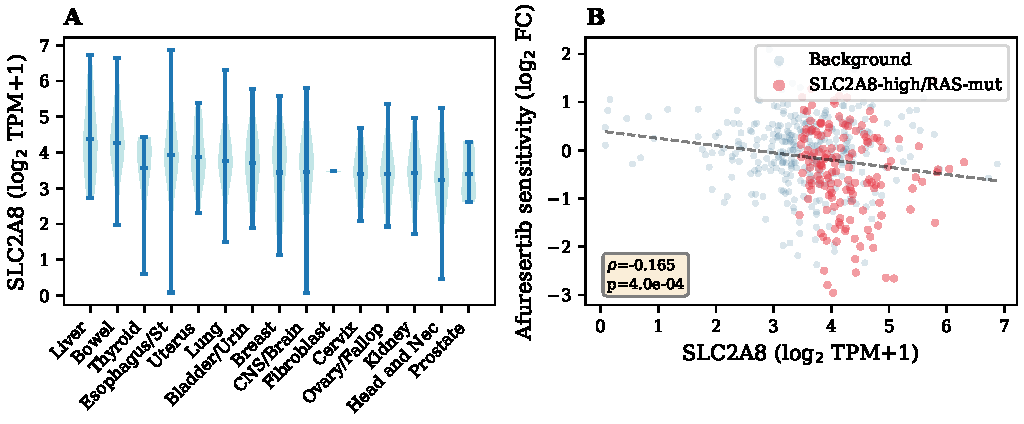
\includegraphics[width=\textwidth]{fig1_slc2a8_landscape.pdf}
\caption{\textbf{SLC2A8 expression landscape and AKT inhibitor
correlation.} (A)~SLC2A8 expression (log$_2$ TPM+1) by lineage across
1,103 cancer cell lines (DepMap 24Q4). Top 15 lineages by median
expression. Pancreatic lineage highlighted in red. (B)~SLC2A8 expression
versus afuresertib (GSK2110183) drug sensitivity. Each point is a cell
line; red points indicate SLC2A8-high/RAS-mutant target group.
Spearman $\rho$ and $p$-value shown.}
\label{fig:landscape}
\end{figure}

\begin{figure}[!ht]
\centering
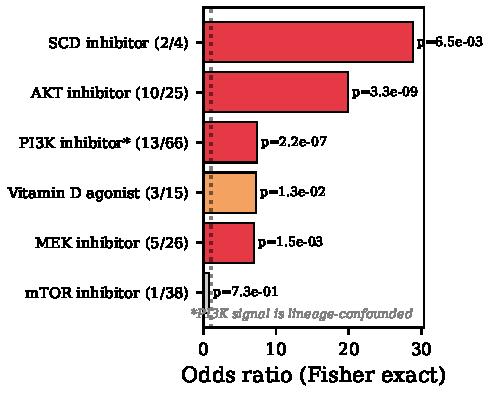
\includegraphics[width=0.5\textwidth]{fig2_moa_enrichment.pdf}
\caption{\textbf{Unbiased PRISM drug screen identifies AKT inhibitors.}
Mechanism-of-action enrichment among compounds with differential
sensitivity in SLC2A8-high/RAS-mutant cells ($p$<0.05) versus background.
Odds ratios from Fisher's exact test. Parentheses show significant/total
compounds per class. Red: $p$<0.01; orange: $p$<0.05; gray: not
significant. *PI3K signal is lineage-confounded (see Figure~3).}
\label{fig:moa}
\end{figure}

\begin{figure}[!ht]
\centering
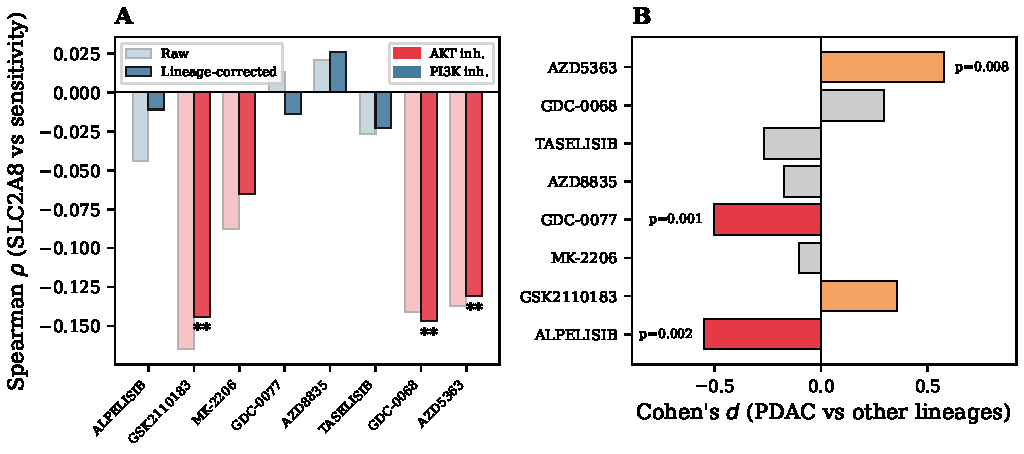
\includegraphics[width=\textwidth]{fig3_lineage_decomposition.pdf}
\caption{\textbf{Lineage decomposition separates AKT signal from PI3K
confound.} (A)~Spearman $\rho$ between SLC2A8 expression and drug
sensitivity before and after lineage correction. Red bars: AKT
inhibitors; blue bars: PI3K inhibitors. ** indicates lineage-corrected
$p$<0.01. AKT signals survive; PI3K signals collapse. (B)~Cohen's $d$
for PDAC lineage effect on each drug's sensitivity, showing that PDAC
cells are inherently sensitive to specific PI3K inhibitors independent
of SLC2A8 expression.}
\label{fig:lineage}
\end{figure}

\begin{figure}[!ht]
\centering
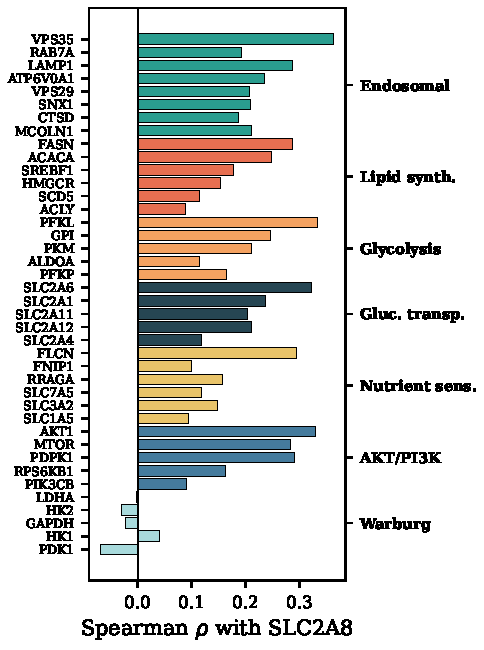
\includegraphics[width=0.5\textwidth]{fig4_metabolic_fingerprint.pdf}
\caption{\textbf{SLC2A8 metabolic co-expression fingerprint.} Spearman
$\rho$ between SLC2A8 and candidate genes across 1,103 cell lines,
organized by metabolic program. The SLC2A8-high subtype co-expresses
endosomal trafficking, lipid synthesis, and oxidative glycolysis genes,
but not Warburg metabolism genes (HK2, LDHA, GAPDH).}
\label{fig:fingerprint}
\end{figure}

\begin{figure}[!ht]
\centering
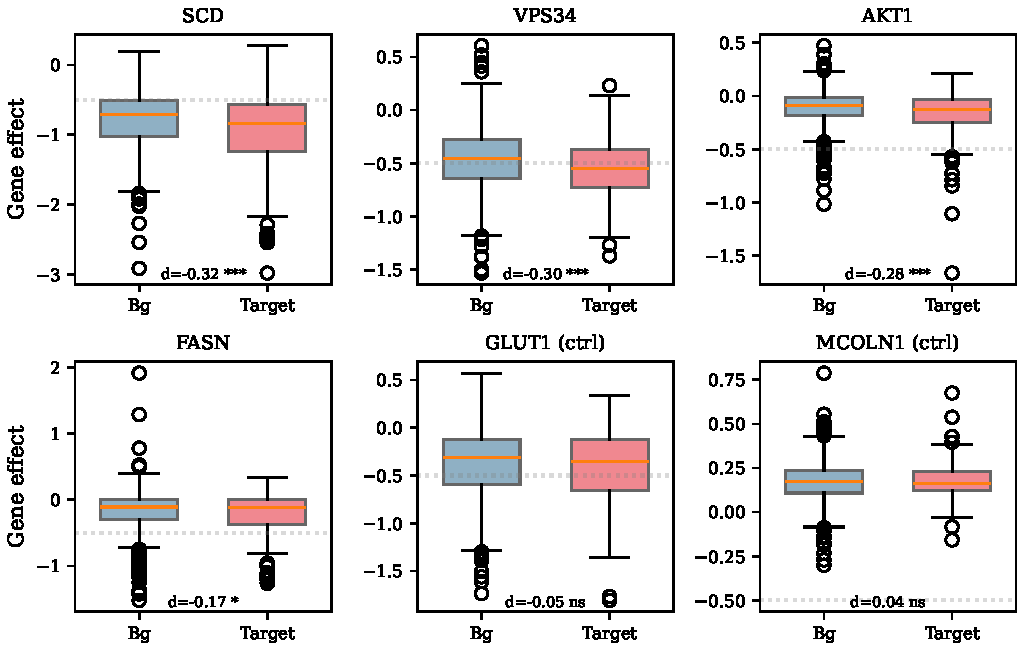
\includegraphics[width=\textwidth]{fig5_crispr_dependencies.pdf}
\caption{\textbf{CRISPR genetic dependencies in SLC2A8-high/RAS-mutant
cells.} Chronos gene effect scores for target (red) versus background
(blue) groups. More negative values indicate greater dependency. SCD,
VPS34 (PIK3C3), AKT1, and FASN show significant differential dependency.
GLUT1 and MCOLN1 shown as negative controls. Cohen's $d$ and
significance indicated.}
\label{fig:crispr}
\end{figure}

\begin{figure}[!ht]
\centering
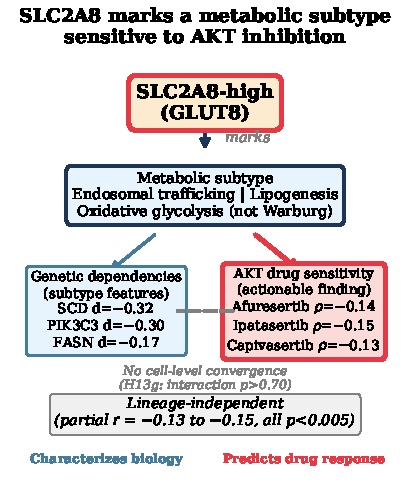
\includegraphics[width=0.5\textwidth]{fig6_model_diagram.pdf}
\caption{\textbf{SLC2A8 marks a metabolic subtype sensitive to AKT
inhibition.} Summary diagram. SLC2A8 expression marks a metabolic
subtype with co-expressed endosomal trafficking, lipogenesis, and
oxidative glycolysis programs. AKT drug sensitivity (right, red) is
the actionable finding; genetic dependencies (left, blue) characterize
the subtype biology. Dashed line indicates that convergence testing
found no cell-level co-occurrence between AKT sensitivity and
lipogenesis dependency (interaction $p$>0.70). Lineage-independent
partial correlations shown at bottom.}
\label{fig:model}
\end{figure}

% ====================================================================
% Bibliography
% ====================================================================
\bibliographystyle{unsrtnat}
\bibliography{references}

% ====================================================================
% Supplementary
% ====================================================================
\clearpage
\appendix
\setcounter{figure}{0}
\renewcommand{\thefigure}{S\arabic{figure}}

\section*{Supplementary Material}

\begin{figure}[!ht]
\centering
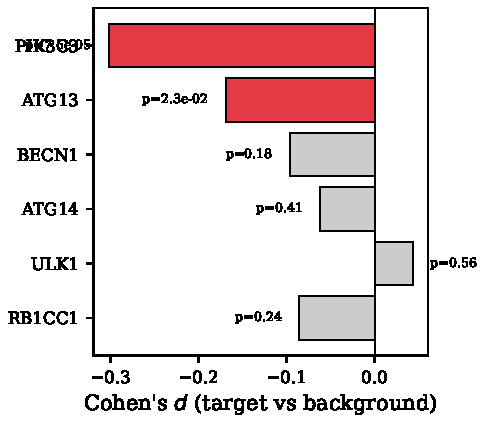
\includegraphics[width=0.5\textwidth]{figS1_pik3c3_decomposition.pdf}
\caption{\textbf{PIK3C3 drives the autophagy initiation signal.}
Cohen's $d$ for CRISPR gene effect (target versus background) across
autophagy initiation genes. PIK3C3/VPS34 dominates the signal. Only
genes with $p$<0.05 are highlighted.}
\label{fig:pik3c3}
\end{figure}

\begin{figure}[!ht]
\centering
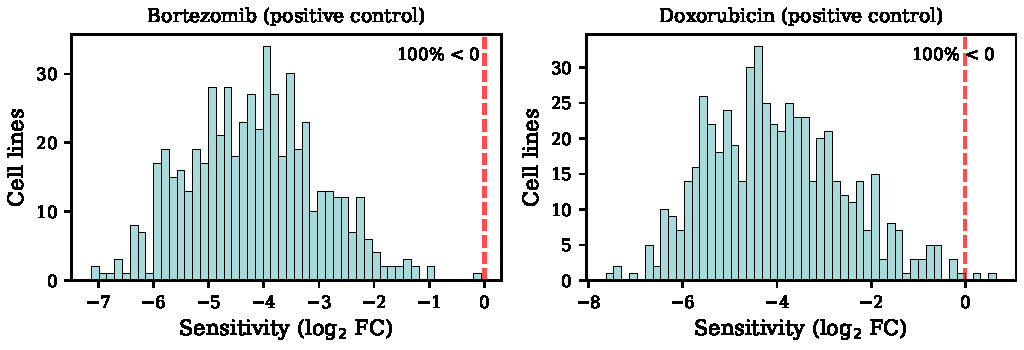
\includegraphics[width=\textwidth]{figS2_prism_sanity.pdf}
\caption{\textbf{PRISM sensitivity sign convention verification.}
Distribution of sensitivity values for bortezomib and doxorubicin
(positive controls). Near-universal negative values confirm that more
negative = greater killing in the PRISM dataset.}
\label{fig:sanity}
\end{figure}

\begin{figure}[!ht]
\centering
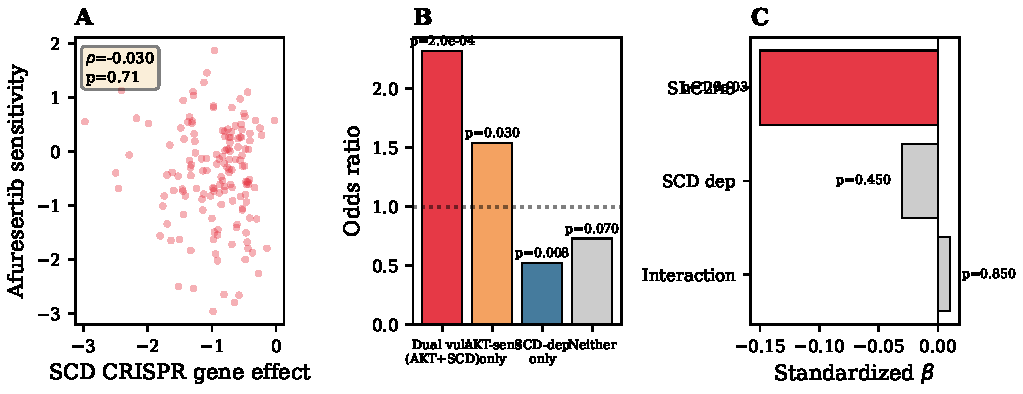
\includegraphics[width=\textwidth]{figS3_convergence.pdf}
\caption{\textbf{Convergence testing: AKT drug sensitivity and
lipogenesis dependency are independently distributed.}
(A)~Scatter plot of SCD CRISPR dependency versus afuresertib drug
sensitivity within SLC2A8-high/RAS-mutant target cells. No
correlation ($\rho$=$-$0.030, $p$=0.72). (B)~Target group
enrichment by vulnerability quadrant. Dual vulnerability (AKT-sens +
SCD-dep) shows group-level enrichment (OR=2.32), but SCD-dep-only is
depleted (OR=0.52), indicating independent marginal enrichments.
(C)~Standardized regression coefficients from the interaction model.
SLC2A8 is the sole significant predictor; SCD dependency and the
interaction term are null.}
\label{fig:convergence}
\end{figure}

\begin{figure}[!ht]
\centering
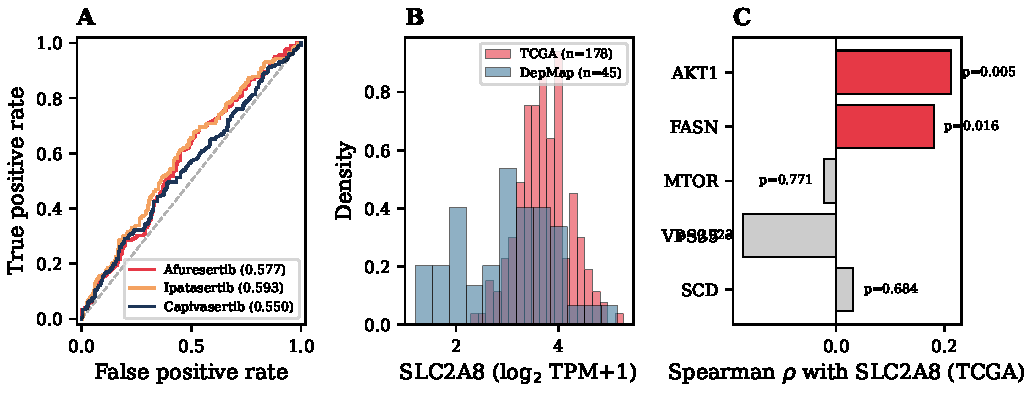
\includegraphics[width=\textwidth]{figS4_roc_tcga.pdf}
\caption{\textbf{Classification performance and TCGA-PAAD validation.}
(A)~ROC curves for SLC2A8 expression predicting above-median AKT
inhibitor sensitivity (afuresertib AUC=0.577, ipatasertib AUC=0.593,
capivasertib AUC=0.550). Dashed line: chance level.
(B)~SLC2A8 expression distribution in TCGA-PAAD tumors (n=178)
versus DepMap PDAC cell lines (n=45). TCGA tumors show higher
expression (KS $p$<0.0001), likely due to stromal contribution.
(C)~SLC2A8 co-expression in TCGA-PAAD patient tumors. AKT1
($\rho$=+0.21, $p$=0.005) and FASN ($\rho$=+0.18, $p$=0.016)
replicate; VPS35 and SCD do not.}
\label{fig:roc_tcga}
\end{figure}

\end{document}
